\chapter{Návrh krytu zařízení}

Stejně jako bylo třeba navrhnout veškerou elektroniku, je zapotřebí vytvořit kryt pro tuto elektroniku. Do tohoto krytu je zapotřebí umístit hlavní desku řídící elektroniky s~nasazenou senzorovou deskou pro měření osvětlení, baterii a~senzor prachových částic. Kryt byl navržen v~programu SOLIDWORKS\footnote{\url{https://www.solidworks.com/}} a~je koncipován pro tisk na 3D tiskárně. 

Kryt je rozdělen na dvě části, kde v~hlavní části je umístěna veškerá elektronika a~poté kryt, který je k~této hlavní části přišroubován. V~krytu nejsou modelovány závity, ale jsou využity mosazné závitové vložky, které se po vytisknutí zahřáté vtlačí do výtisku. Toto řešení má výhodu ve snadné rozebiratelnosti a~také je pevnější než přímé zašroubování do plastu. Stejným způsobem je přišroubována také hlavní deska. Pro připevnění senzoru prachových částic a~baterie je využito možností 3D tisku a~jsou tedy drženy pouze vložením do předem vymodelovaných pozic a~poté přidrženy krytem celé krabičky. Navržená krabička je vidět na obrázku \ref{fig_Case}.

\begin{figure}[h]
    \centering
    \subfloat[][Spodní strana krabičky]{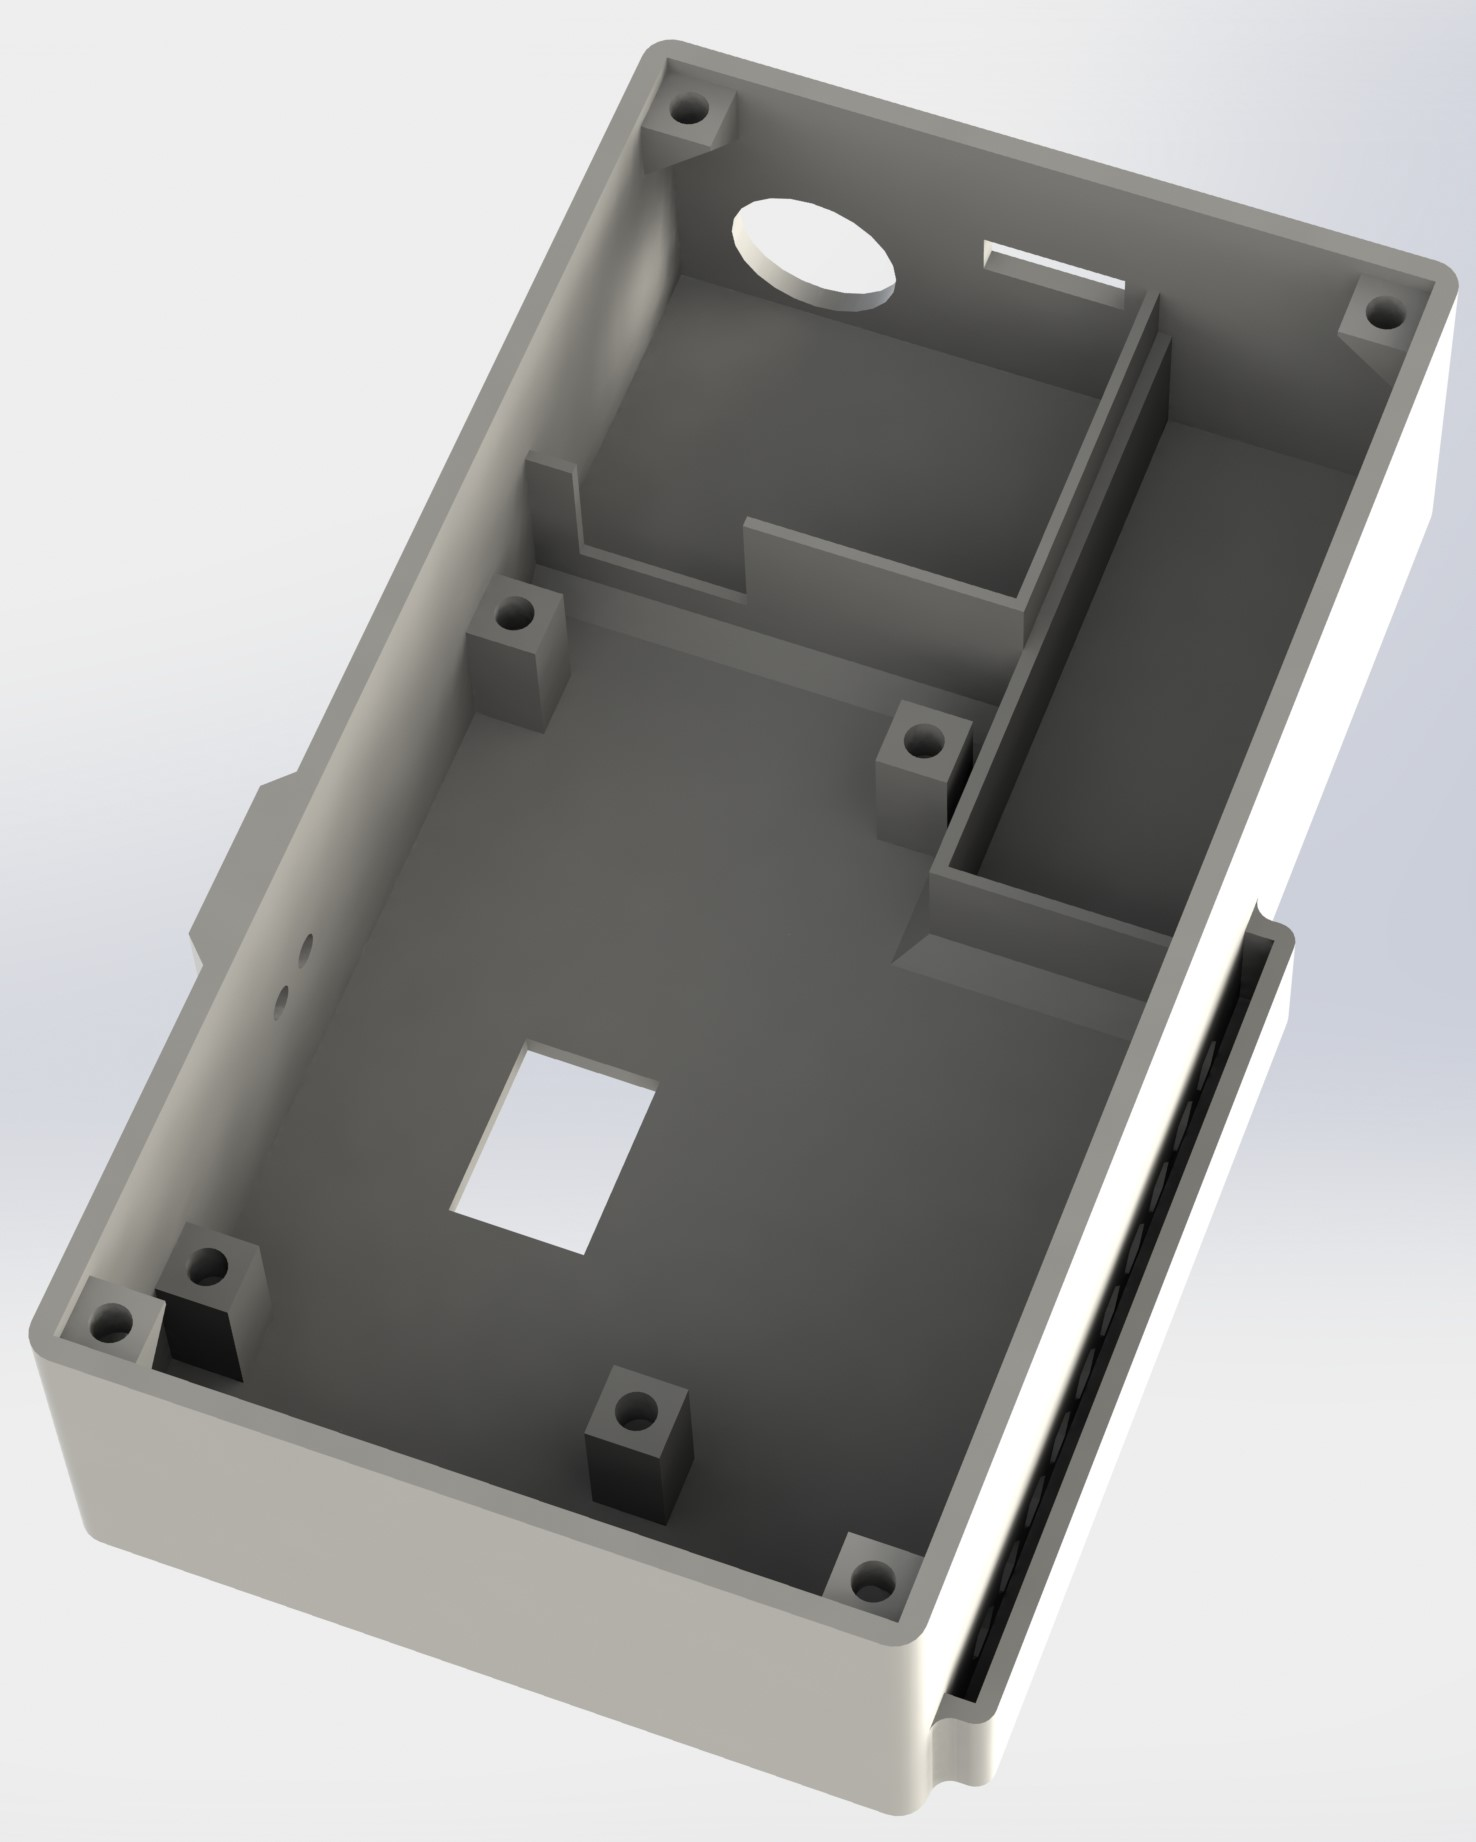
\includegraphics[width=0.55\textwidth]{obrazky/case_bot.JPG}}
    \quad
    \subfloat[][Horní strana krabičky]{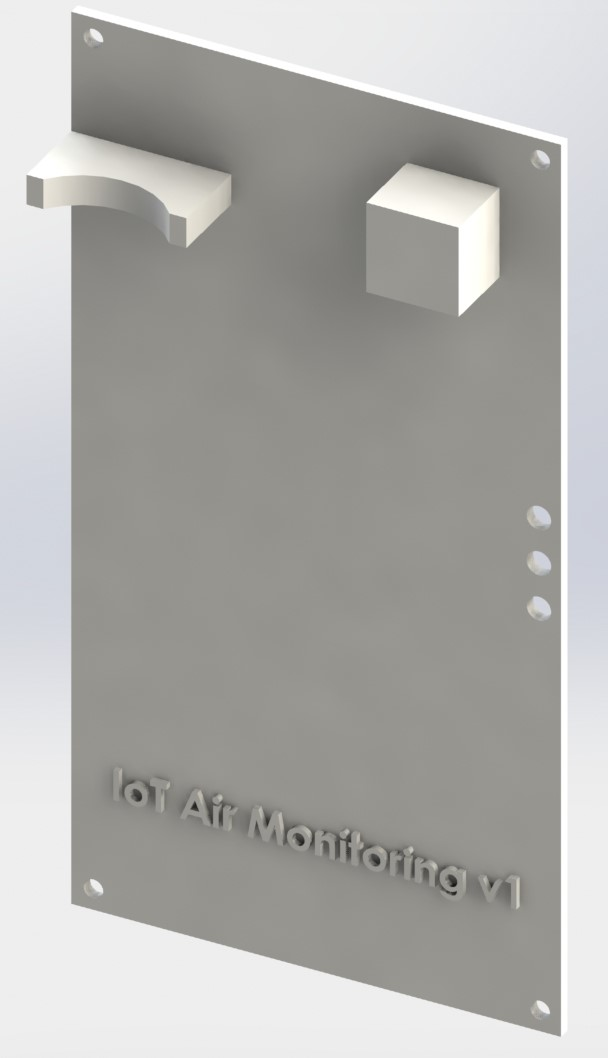
\includegraphics[width=0.39\textwidth]{obrazky/case_top.JPG}}
    \caption{3D model krabičky pro elektroniku.}
    \label{fig_Case}
\end{figure}